\begin{frame}
  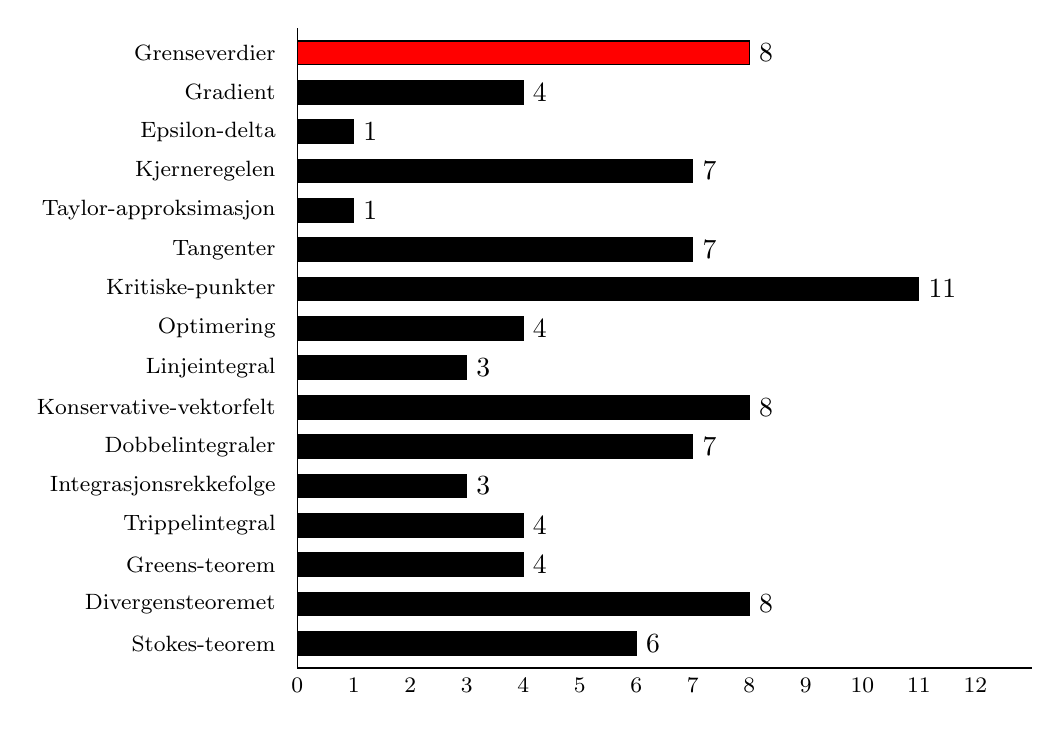
\begin{tikzpicture}
    \begin{axis}[ xbar=0pt, /pgf/bar shift=0pt, legend style={ legend columns=4,
        at={(xticklabel cs:0.5)}, anchor=north, draw=none }, ytick={0,...,15},
      ytick style={draw=none},% <- added
      axis y line*=none, axis x line*=bottom, tick label
      style={font=\footnotesize}, legend style={font=\footnotesize}, label
      style={font=\footnotesize}, xtick style={draw=none},% <- added
      xtick={0,1,...,12}, width=.9\textwidth, bar width=3mm, y dir = reverse,
      xmin=0, xmax=13, area legend,
      y=5mm, enlarge y limits={abs=0.625},
      style={text=black}, every axis plot/.append style={fill},
      nodes near coords, nodes near coords,
      yticklabels={%
        {\topicref{Grenseverdier}},
        {\topicref{Gradient}},
        {\topicref{Epsilon-delta}},
        {\topicref{Kjerneregelen}},
        {\topicref{Taylor-approksimasjon}},
        {\topicref{Tangenter}},
        {\topicref{Kritiske-punkter}},
        {\topicref{Optimering}},
        {\topicref{Linjeintegral}},
        {\topicref{Konservative-vektorfelt}},
        {\topicref{Dobbelintegraler}},
        {\topicref{Integrasjonsrekkefolge}},
        {\topicref{Trippelintegral}},
        {\topicref{Greens-teorem}},
        {\topicref{Divergensteoremet}},
        {\topicref{Stokes-teorem}}}]
      \addplot[fill=red] coordinates {(8,0)};
      \addplot[fill=black] coordinates {(4,1)};
      \addplot[fill=black] coordinates {(1,2)};
      \addplot[fill=black] coordinates {(7,3)};
      \addplot[fill=black] coordinates {(1,4)};
      \addplot[fill=black] coordinates {(7,5)};
      \addplot[fill=black] coordinates {(11,6)};
      \addplot[fill=black] coordinates {(4,7)};
      \addplot[fill=black] coordinates {(3,8)};
      \addplot[fill=black] coordinates {(8,9)};
      \addplot[fill=black] coordinates {(7,10)};
      \addplot[fill=black] coordinates {(3,11)};
      \addplot[fill=black] coordinates {(4,12)};
      \addplot[fill=black] coordinates {(4,13)};
      \addplot[fill=black] coordinates {(8,14)};
      \addplot[fill=black] coordinates {(6,15)};
    \end{axis}
  \end{tikzpicture}
\end{frame}

\begin{frame}
  \frametitle{Grenseverdier}
  \section{Grenseverdier}
  \label{subsec:Grenseverdier}
  En funksjon $f(x,y)$ er kontinuerlig i $(0,0)$ dersom
  %
  \begin{equation*}
    \lim_{(x,y)\to(0,0)} f(x,y) = f(0,0)\,,
  \end{equation*}
  %
  \emph{uavhengig} av hvilken retning du nærmer deg origo. \visible<2->{Anta du ønsker å undersøke
  om en funksjon på formen
  %
  \begin{equation*}
    f(x,y) :=
    \begin{cases}
      \frac{g(x,y)}{h(x,y)}, & \text{når} \quad (x,y) \neq (0,0), \\
      0, & \text{når} \quad (x,y) = (0,0)
    \end{cases},
  \end{equation*}
  er kontinuerlig.
  \begin{itemize}
    \item Forenkle $f(x,ax^b)$ mest mulig. Eksisterer $a$ og $b$
      slik at $\lim_{x \to 0}f(x,ax^b) \neq f(0,0)$? Da er funksjonen
      \emph{ikke} kontinuerlig.
    \item Inneholder $h(x,y)$ uttrykket $x^2 + y^2$? Forenkle $f(r \cos \theta,
      r \sin \theta)$. Undersøk om $\lim_{r \to 0} f(r \cos \theta, r\sin
      \theta) = 0$ for \emph{alle} vinkler, altså $\theta$.
  \end{itemize}}
\end{frame}

\begin{frame}
  \begin{oppgave}{V2016, Oppgave 1}
    %
    \begin{equation*}
      f(x,y) :=
      \begin{cases}
        \cfrac{yx^3}{3y^2 + x^6}, & \text{når} \quad (x,y) \neq (0,0), \\
        0, & \text{når} \quad (x,y) = (0,0)
      \end{cases}.
    \end{equation*}
    %
    Forklar hvorfor $f$ ikke er deriverbar i $(0,0)$, men de partiellderiverte
    $\diffp{f}{x}(0,0)$ og $\diffp{f}{y}(0,0)$ eksisterer.
  \end{oppgave}
    \only<1-4>{\textbf{Steg 1:} Forenkle $f(x,ax^b)$ mest mulig.}
   \only<5-7>{\textbf{Steg 2:} Eksisterer det nå en $a$ og $b$ slik at $\displaystyle\lim_{x \to 0} f(x, ax^b)
     \neq f(0,0) = 0$?}
   %
   \only<1-7>{
  \begin{equation*}
    \only<6->{\lim_{x\to 0}}\only<1-5>{f(x, ax^b)}\only<6->{f(x,ax^3)}
    \only<1>{= \frac{ax^bx^3}{3(ax^b)^2+x^6}}
    \only<2>{= \frac{ax^{3+b}}{3a^2x^{2b} + x^6}}
    \only<3>{= \frac{a}{3a^2x^{2b-(3+b)} + x^{6 - (3+b)}}}
    \only<4-5>{= \frac{a}{3a^2x^{b-3} + x^{3 - b}}}
    \only<6>{= \lim_{x \to 0} \frac{a}{3a^2x^{3-3}+x^{3-3}}}
    \only<7>{= \frac{a}{3a^2 + 1}}
  \end{equation*}}
  %
  \only<7>{Siden $f$ ikke er kontinuerlig kan den naturlig nok heller ikke være
    deriverbar!}
  \only<8>{%
    \begin{itemize}
        \item Notasjonen $\diffp{f}{x}(0,0)$ betyr \emph{ikke} den deriverte med
    hensyn på $x$ i origo!

    \item Den partiellderiverte er den \emph{retningsderiverte} av $f$ i retning
        $(1,0)$ altså langs $x$-aksen. Tilsvarende for $\partial f/\partial y(0,0)$.

   \item At funksjonen ikke er deriverbar betyr at det eksisterer en retning mot origo
 hvor den retningsderiverte ikke har et klart definert stigningstall. De
        retningsderiverte i $x$ og $y$ retningen kan såklart likevell eksistere.
    \end{itemize}}
  \only<9-12>{%
    Den \emph{retningsderiverte} til $f$ i punktet $\A=(0,0)$ og
    \emph{retning} $\rr$ er gitt ved
    \begin{align*}
      f'(\A; \rr) & = \lim_{h \to 0} \frac{f(\A + h \rr) - f(\A)}{h}\\
      \diffp{f}{x}(0,0) & =
      \only<9>{\lim_{h \to 0} \frac{f((0,0) + h (1,0)) - f(0,0)}{h}}
      \only<10>{\lim_{h \to 0} \frac{f(h,0) - f(0,0)}{h}} 
      \only<11>{\lim_{h \to 0} \frac{\frac{0\cdot h^3}{3\cdot 0^2 + h^6} - 0}{h}} 
      \only<12>{\lim_{h \to 0} \frac{0 - 0}{h} = 0} \\
      \diffp{f}{y}(0,0) & =
      \only<9>{\lim_{h \to 0} \frac{f((0,0) + h (0,1)) - f(0,0)}{h}}
      \only<10>{\lim_{h \to 0} \frac{f(0,h) - f(0,0)}{h}}
      \only<11>{\lim_{h \to 0} \frac{\frac{h \cdot 0^3}{3h^2 + 0^6} - 0}{h}} 
      \only<12>{\lim_{h \to 0} \frac{0 - 0}{h} = 0} 
    \end{align*}
  }
\end{frame}

\begin{frame}
  \begin{oppgave}{K2013, Oppgave 3}
    Vis at en av grensene under eksisterer mens den andre ikke gjør det
    %
    \begin{equation*}
      \lim_{(x,y)\to(0,0)} \frac{xy}{\sqrt{x^2+y^2}}
      \qquad
      \lim_{(x,y)\to(0,0)} \frac{xy}{x^2+y^2}
    \end{equation*}
  \end{oppgave}
  \only<1-4>{\textbf{Steg 1}: Uttrykket inneholder $x^2 + y^2$ så vi forenkler $f(r \cos
    \theta, r \sin \theta)$.}
  \only<5-6>{
  \textbf{Steg 2}: Undersøker om $\lim_{r \to 0} f(r \cos \theta, r\sin \theta)$ er uavhengig av $\theta$.} 
  \begin{align*}
  \only<1>{
    & \ \frac{(r\cos \theta) (r\sin \theta)}{\sqrt{(r\cos \theta)^2 + (r\sin \theta)^2}\,}
    && \ \frac{(r \cos \theta)(r\sin \theta)}{(r \cos \theta)^2 + (r \sin \theta)^2}}
       \only<2>{
     & \ \frac{r^2(\cos \theta) (\sin \theta)}{\sqrt{r^2(\cos^2\theta + \sin^2\theta)}\,}
    &&  \ \frac{r^2(\cos \theta)(\sin \theta)}{r^2(\cos^2\theta + \sin^2\theta)}}
       \only<3>{
     & \ \frac{r^2}{\sqrt{r^2}}(\cos \theta)(\sin \theta)
    && \ \frac{r^2}{r^2}(\cos \theta)(\sin \theta)}
       \only<4>{
    & \ r (\cos \theta)(\sin \theta)
    && \ (\cos \theta)(\sin \theta)}
       \only<5>{
    \lim_{r \to 0} & \ r (\cos \theta)(\sin \theta)
    && \lim_{r \to 0} \ (\cos \theta)(\sin \theta)}
              \only<6>{
    \underbrace{\lim_{r \to 0} \ r (\cos \theta)(\sin \theta)}_{\text{Ja, $0$ for alle $\theta$}}
    && \underbrace{\lim_{r \to 0} \ (\cos \theta)(\sin \theta)}_{\text{Nei, $\theta=0 \to 0$, $\theta=\pi/4 \to 1/2$.}}}
  \end{align*}
\end{frame}


%%% Local Variables:
%%% mode: latex
%%% TeX-master: "main"
%%% End:
